近年,ナレッジマネジメントが企業経営の重要な要素と言われ,
導入する企業が増えている.
ナレッジマネジメントとは,個人の持つ知識や情報を組織全体で共有し,
有効に活用することで業績を上げようという経営手法である.
日本語では,「知識管理」などと訳され,「KM」と略されることもある.
参考文献1(\verb|http://e-words.jp/w/|ナレッジマネジメント.html)

ナレッジマネジメントでは,グループ開発において共有する知識は
暗黙知と形式知に分けられる.
暗黙知は主に口伝によって一対一でつたえられたり,あるいは体で覚えるというのが一般的である.
しかし,定着するまでの間は一般的にメモという形で個人的な知識として扱われるのが普通である.
一方で図書館やwebなどでは文書やhyper textとして誰もが読める形で保管,提供される.
これらは形式知と呼ばれる.(図1 暗黙知,形式知)

暗黙知の形式知化はいくつも行われている.
google検索でよく引っかかるQiita.comやcheatgraphy.comなどもそれらをまとめるサイトを提供している.
また,デザインパターンも「プログラマが持っていた暗黙知に名前をつけることで形式知化した」と
ruby開発者のまつもとゆきひろも指摘している\verb|{{fn'デザインパターン,コード解説'}}|.
ある意味,暗黙知の形式知化をいかに効率よく行うかは知識共有の最大の目的とも言える.

このような暗黙知と形式知を提供するフォーマットはそれぞれの特徴を引き出すためにそれぞれ異なった
フォーマットで記述されている.

\begin{itemize}
\item 暗黙知は主にメモとして保存しやすいように単純なテキスト形式が取られる.
\item web発信においては,複雑な構文となるhyper textではなく,手軽にwebサイトを構築するwikiに対応したmark up言語が取られる.また,
\item 書籍としては,体裁,数式の綺麗さだけでなく,目次,索引,引用文献などの自動作成の観点からlatexで書かれることが多い.
\end{itemize}
しかし,それぞれを別々に書いていては,一箇所に修正があるとすべてのフォーマットに対して行う必要が出てくる.
これはプログラマの心得の核心をなす「DRY(Don't Repeat Yourself)」原則を
破ることとなる\verb|{{fn('pragmatic programmer')}}|.
プログラマはこれらの変換を自動化するコンバータを作成して,一箇所の修正によって
他のフォーマットでの修正に反映されるように,自動的に行うシステムを構築している.

本研究においては,図\ref{knowledge\_controll\_cui}に示した通り,西谷研で活用しているメモソフト
my\_help,wiki cloneのhiki, およびlatexの間を自動変換するシステムの開発を目的としている.

\begin{figure}[htbp]\begin{center}
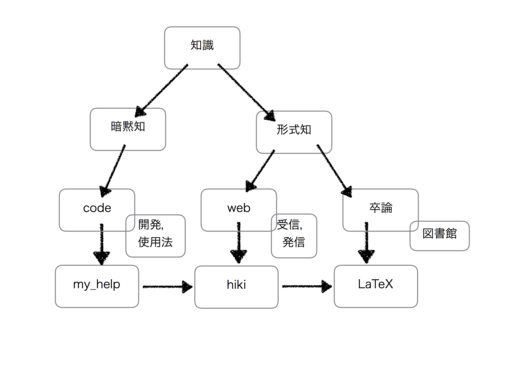
\includegraphics[width=6cm,bb=0 0 442 500]{../figs/./knowledge_controll_cui.png}
\caption{}
\label{default}\end{center}\end{figure}
\begin{table}[htbp]\begin{center}
\caption{}
\begin{tabular}{ll}
\hline
\fig{knowledge\_controll\_cui} 知識の分類と,それぞれに適合したシステムおよびフォーマット.  \\ \hline
\hline
\end{tabular}
\label{default}
\end{center}\end{table}
%for inserting separate lines, use \hline, \cline{2-3} etc.

